\chapter{Perspectives et bilan}
\label{sec:Ending}
% Ce que nous avons fait
% Notre ressenti
% Y a t'il une place pour d'autres filtres de rehaussement ?
% Le rehaussement a t'il un futur ?

\section{Bilan du rehaussement}

Dans les chapitres précédents, nous avons couvert l'ensemble de nos travaux sur l'analyse des filtres de rehaussement. Pour ce chapitre, nous proposons un bilan sur le rehaussement de vaisseaux et proposons des perspectives concernant leur utilisation, issues d'expérimentations réalisées durant la seconde moitié de la thèse. 

%\subsection{Rehaussement et deep learning}

%Nous n'avons pas encore abordé la question de la place du rehaussement parmi les méthodes de segmentation populaires actuellement. En effet, le deep learning a pris une place très importante dans la littérature d'aujourd'hui, en particulier les réseaux \textit{end-to-end} qui intègrent l'ensemble des traitements menant à la segmentation. Ces réseaux apprennent leur propre modèle interne et extraient leurs propres caractéristiques pour définir leur propre critère de segmentation. On peut donc se légitimement s'interroger sur la nécessité d'incorporer des filtres de rehaussement aux réseaux de neurones.

%Comme nous l'avons présenté dans le chapitre 3, les filtres de rehaussement de vaisseaux viennent en amont de la segmentation. On peut donc également les utiliser en amont d'un réseau de neurones. Les performances du deep learning sont largement influencées par le type de données qui lui sont présentées. On cherche notamment à ce qu'une base de données soit la plus représentative du problème que l'on cherche à traiter. Plusieurs méthodes d'intégrations des filtres de rehaussement sont possibles. La première méthode consiste à filtrer une base de données initiale et de présenter au réseau les données filtrées. On peut alors espérer guider l'apprentissage du réseau en mettant en valeur les structures tubulaires et en éliminant les autres structures.

\subsection{Futur du rehaussement}
%deep 
Ces dernières années, le deep learning est devenu la technologie la plus explorée pour résoudre des tâches complexes de segmentation. En particulier,  on privilégie les méthodes de bout en bout (\textit{end-to-end}). Ces méthodes concentrent toute la chaîne de traitement dans un réseau de neurones. Celui-ci apprend de lui-même à élaborer un modèle, à extraire des caractéristiques et à segmenter un organe. Comme on a pu le voir précédemment, le rehaussement s'applique en amont des chaînes de traitement de la segmentation et il peut donc aussi s'appliquer en amont des réseaux de neurones. Le traitement des jeux de données en deep learning est particulièrement important, puisque dans ces systèmes, c'est le jeu de données qui va contrôler la capacité du réseau à se spécialiser sur un problème ou au contraire à le généraliser. Un jeu de données se doit donc d'être le plus représentatif du problème que l'on cherche à traiter.

Les filtres de rehaussement de vaisseaux peuvent faciliter cette représentativité, puisqu'ils permettent de mettre en valeur les vaisseaux tout en éliminant une partie des autres structures. On peut, de plus, utiliser différents filtres ou différentes paramétrisations pour augmenter artificiellement nos données ou renforcer l'apprentissage de vaisseaux spécifiques.
% deep + vesselness

Nous avons effectué un travail collaboratif \cite{Affane_2022_article_commun} dans le cadre du projet ANR avec Abir Affane et al. où nous avons fait l'expérience de tester plusieurs combinaisons de filtres de rehaussement (Jerman, Sato, RORPO et Zhang) et d'architectures de réseaux de neurones (U-net, Dense Net, MultiRes U-net). Les expériences ont été menées sur la base de l'Ircad avec les filtres optimisés dont les paramètres optimaux ont été trouvés par notre banc de test. Les résultats des expériences montrent que le rehaussement, en particulier le rehaussement homogène de Jerman peut aider les réseaux à mieux segmenter les vaisseaux. En particulier, l'usage des filtres montre son efficacité lorsque les réseaux sont entrainés sur des données plus réduites. Nous avons illustré ce cas en entrainant les réseaux avec des blocs (couches d'un volume de quelques voxels d'épaisseurs) plutôt qu'avec des volumes entiers. Survarachakan et al. \cite{Survarachakan2021_deep_vesselness} ont proposé des travaux similaires qui valident, eux aussi, l'utilisation des filtres de rehaussement afin d'améliorer la segmentation de réseaux de type U-net.

Les réseaux de neurones sont d'ailleurs connus pour avoir du mal à généraliser d'une modalité à une autre. En effet, l'apparence des vaisseaux peut changer selon les modalités ainsi que le contexte alentour. Les sorties des filtres de rehaussement ont aussi l'avantage d'être définis dans un domaine relativement homogène. On peut donc imaginer se servir des filtres de rehaussement pour unifier les modalités. On pourrait ainsi créer des jeux de données mixtes contenant des résultats de filtrages issus de modalités différentes et ainsi améliorer la généralisation des réseaux.

Une autre manière d'utiliser les filtres de rehaussement avec le deep learning est de considérer le résultat d'un filtrage comme un nouveau canal de l’image par analogie avec les images multi-spectrales. Ainsi, au lieu de remplacer les volumes présentés aux réseaux par des volumes filtrés, on concatène aux données initiales plusieurs filtrages. Un vaisseau est ainsi décrit par son aspect initial ainsi que par plusieurs types de rehaussements qui fournissent des données complémentaires. Lors de l'apprentissage, un réseau de neurones pourrait alors choisir la combinaison d'informations qui lui permettrait de segmenter au mieux les vaisseaux. \newV{L'usage de données multispectrales est utilisée avec succès dans d'autres domaines tel que l'apprentissage compressé pour la classifcation de maladies des plantes \ref{Douarre2019_ctis}.}

\subsection{Amélioration du rehaussement}

Une autre question est la place de nouveaux filtres de rehaussement dans la littérature. Notre avis sur la question est que les filtres existants offrent une solution à une bonne partie des problèmes rencontrés par le rehaussement. Toutefois, les avantages des filtres sont dispersés à travers un certain nombre d'entre eux. Par exemple, la gestion du bruit proposé par le filtre de Frangi est particulièrement efficace tout comme la manière d'homogénéiser le rehaussement proposé par Jerman. Ces deux propriétés mériteraient d'être regroupées dans un seul filtre. On disposerait ainsi d'un filtre similaire à celui de Jerman qui serait plus résistant au bruit. Nous n'avons pas étudié le cadre de OOF de manière extensive, mais celui-ci mériterait d'être testé avec des mesures de tubularité plus élaborées (Frangi, Sato, Jerman, etc.) afin d'évaluer plus précisément le débordement du filtre par rapport à la taille réelle des vaisseaux.

Enfin, il est envisageable de proposer un filtre de rehaussement basé sur un apprentissage à base de deep learning, cependant il est difficile de cerner l'apport qu'aurait une telle méthode par rapport à des réseaux qui effectuent directement de la segmentation. Par exemple un réseau Unet, produit une carte de probabilité presque binaire puisque les vérités terrains sont des segmentations. Produire un réseau de neurones qui prédit un rehaussement demanderait une vérité terrain du rehaussement attendu. La vérité terrain de vaisseaux, en termes de carte de rehaussement, est encore plus difficile à définir qu'une segmentation manuelle. De plus, dans le cas où l'on utiliserait un filtre existant comme vérité terrain, le réseau issu de l'entrainement ne permettrait pas forcément de dépasser les limitations intrinsèques du filtre utilisé.

Nous l'avons relevé plusieurs fois dans notre manuscrit, produire des annotations est une tâche critique pour le développement de nouveaux algorithmes de segmentation des vaisseaux. Cependant, on ne peut pas demander à des médecins de mobiliser des heures consacrées à l'annotation de volumes alors quelles pourraient être consacrées à prendre soin des patients. Le manque de personnel dans les hôpitaux ne semble pas indiquer une amélioration prochaine de cette situation. La gestion toujours plus stricte des données médicales n'aide pas non plus à faciliter de telles collectes et annotations de données. Ces observations prennent à contre-pied la tendance du deep learning à exploiter toujours plus de données.

Nous avons tenté une approche qui cherche à réduire au minimum le temps passé à annoter un volume. En effet, la communauté est plus à même d'obtenir des bases de données annotées si le temps d'annotation passe de 30 à 60 minutes à une dizaine de minutes. Dans un réseau vasculaire, il n'existe vraiment qu'un seul type de points remarquables : les bifurcations. Celles-ci correspondent par définition à l'embranchement entre plusieurs vaisseaux. Dans un réseau vasculaire en forme d'arbre comme dans le foie, une bifurcation est formée par le départ de deux vaisseaux en aval et à la terminaison d'un vaisseau en amont. Elle peut donc servir de point de départ pour des algorithmes de suivi de vaisseaux. De plus, si l'on considère que le médecin ne doit positionner qu'un seul point au centre de chaque bifurcation, le temps d'annotation s'en trouve drastiquement réduit. En comparaison, une segmentation des vaisseaux nécessite d'annoter l'ensemble des pixels des vaisseaux.
 
Une identification des vaisseaux à partir des bifurcations revient donc à :

\begin{itemize}
\item localiser les bifurcations ;
\item construire une hiérarchie entre les bifurcations ;
\item extraire le réseau vasculaire (ligne centrale ou segmentation).
\end{itemize}

Une solution envisée pour l'extraction du réseau vasculaire pourrait être de relier les bifurcations deux à deux grâce à un parcours de chemin. On pourrait alors optimiser le chemin en fournissant à l'algorithme une carte de coût qui serait le résultat d'un filtre de rehaussement de vaisseaux. En prenant un filtre dont le rehaussement est dégressif sur les bords (Frangi, Sato, Jerman $\tau > 0.5$) on peut favoriser les chemins passant par le centre des vaisseaux. Si l'on veut aller plus loin, on peut même en partie reconstruire les vaisseaux en estimant leur rayon à partir de la ligne centrale.

Le défi ici est donc la détection et la localisation des bifurcations. En termes de modélisation, les bifurcations sont difficiles à définir. On considère d'habitude les bifurcations comme des zones en forme de blob, c'est-à-dire où le gradient s'éloigne du centre dans toutes les directions. Cette hypothèse est plus fragile lorsqu'elle est confrontée à la réalité des cas pratiques. Par exemple, si les vaisseaux composant la bifurcation ne font pas la même taille, la zone non tubulaire identifiant la bifurcation se trouve déportée sur les bords des vaisseaux et la géométrie se trouve plus aplatie que circulaire (Fig. \ref{fig:gradient_shift}). 

\begin{figure}[ht]
    \centering
    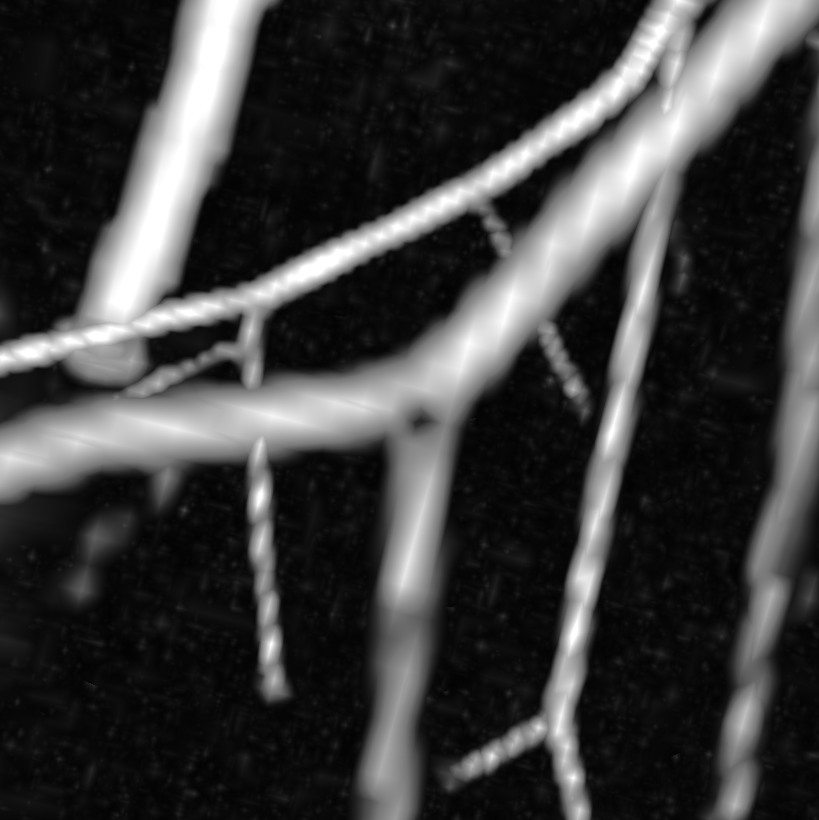
\includegraphics[height=5cm]{Images/Vascu_2_k_Sato.png}
    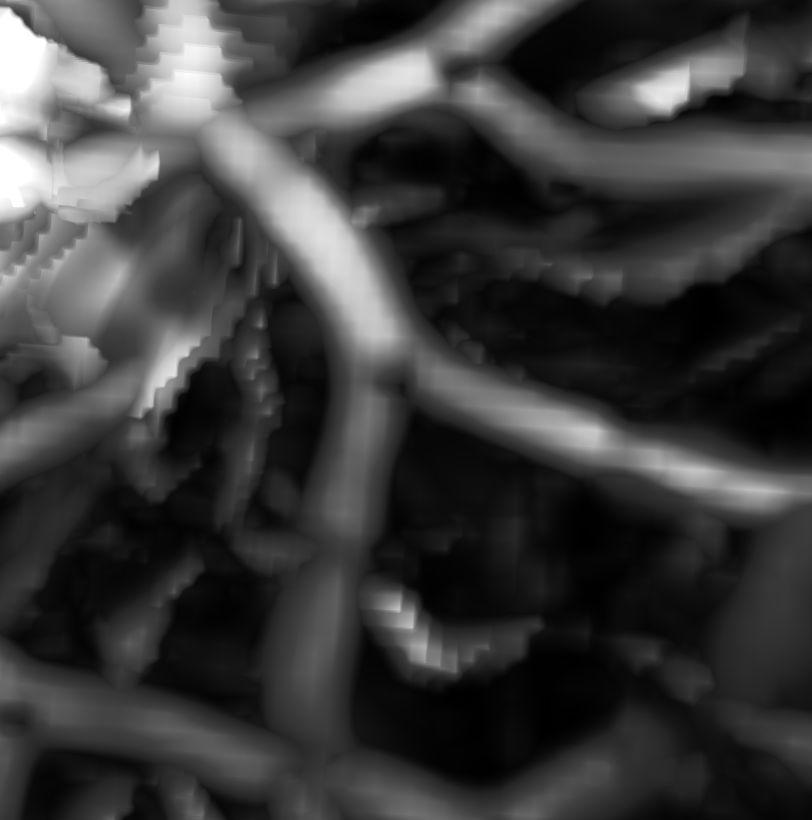
\includegraphics[height=5cm]{Images/Ircad_k_Sato.png}
    \caption{Filtre de Sato présentant une perte de signal marquée dans les zones non tubulaires, correspondant ici aux bifurcations. Lorsque les vaisseaux ne sont pas de même taille, la perte de signal ne se situe pas au centre, mais sur les bords du vaisseau principal.}
    \label{fig:gradient_shift}
\end{figure}


Par conséquent, la variabilité des bifurcations les rend difficile à modéliser par un filtre de rehaussement. Jerman et al. ont proposé un filtre de rehaussement pour les anévrismes (blobs) \cite{Jerman2015_blobness}, mais ils ont dû compléter la méthode par un système de visualisation particulier, car les blobs sont rehaussés de manière non homogène. Ce filtre appliqué à la détection des bifurcations dans VascuSynth ne détecte pas bien les bifurcations. Au contraire, les extrémités des vaisseaux ressemblant à des anévrismes sont rehaussés.

Nous avons aussi testé une combinaison de filtres. Nous avons en effet constaté que le filtre de Sato, lorsque que $\alpha_1$ était bas, provoquait des trous bien visibles dans la réponse des bifurcations. Nous avons essayé de différencier le manque de signal des bifurcations du manque de signal dans les régions homogènes (vides) en effectuant une différence entre le filtre de Sato et le filtre de Jerman (Fig. \ref{fig:subtract_vesselness}). Deux problèmes apparaissent alors. Un résidu de signal est présent aux bifurcations, mais la délimitation de celui-ci est très variable, formant parfois des structures plates plutôt que sphériques, confirmant nos observations précédentes. De plus, le filtre de Jerman estime le rayon des vaisseaux de manière plus large que le filtre de Sato. En faisant la différence $\textrm{Jerman}-\textrm{Sato}$ on se retrouve avec un résultat dont la géométrie interne serait comparable à celle d'un bambou, avec une seule composante connexe qui entoure les vaisseaux (chambres d'air) et séparée en compartiment par des jonctions mal délimitées correspondant aux bifurcations.

\begin{figure}[ht]
    \centering
    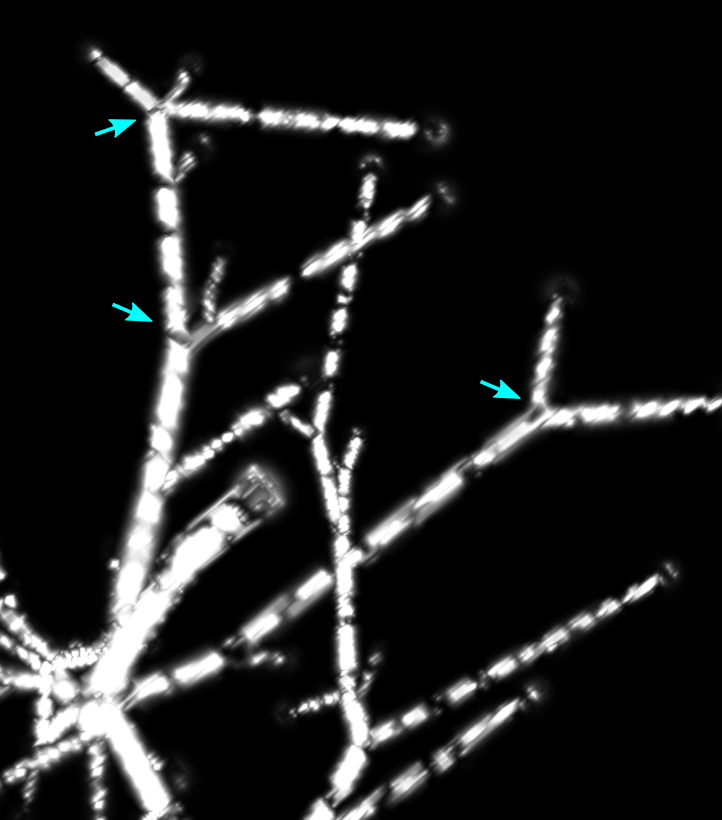
\includegraphics[height=4cm]{Images/SatoFilter_bif.png}
    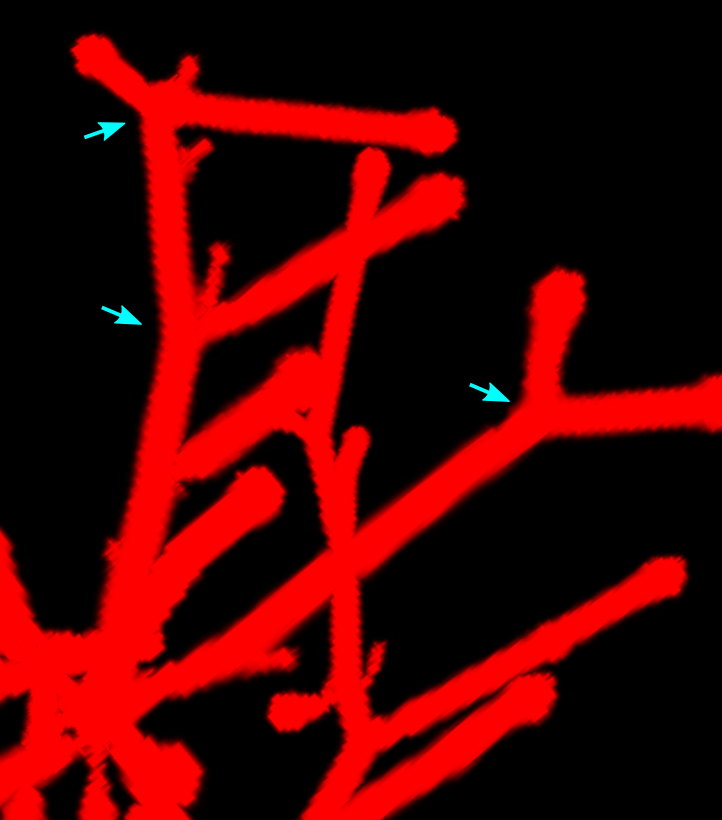
\includegraphics[height=4cm]{Images/JermanFilter_bif.png}
    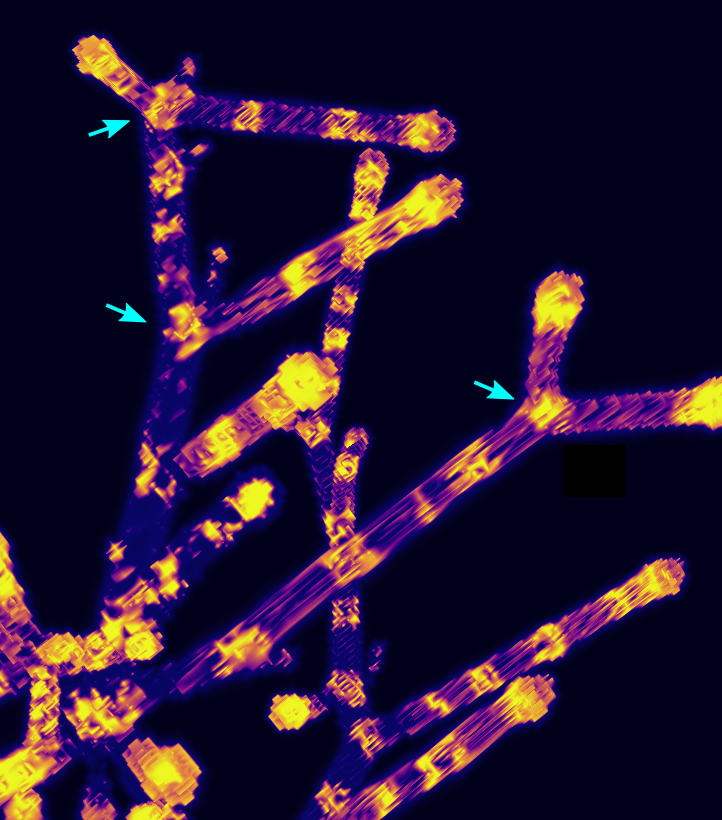
\includegraphics[height=4cm]{Images/subJermanSato_bif.png}
    \caption{Filtre de Sato (Blanc), Filtre de Jerman (Rouge), différence $\textrm{Jerman}-\textrm{Sato}$ (jaune). Bien que le signal du rehaussement soit plus fort sur les bifurcations, la visualisation en coupe montre une exploitation difficile de cette méthode.}
    \label{fig:subtract_vesselness}
\end{figure}

Face à la variabilité des bifurcations, nous nous sommes tournés vers le deep learning afin de développer une méthode résistante aux variations de géométrie.

L'ensemble de nos expériences ont été réalisées avec des jeux de données synthétiques VascuSynth dont on connait la position des bifurcations.

Nous avons d'abord tenté de segmenter les bifurcations en utilisant comme vérité terrain les masques des bifurcations que nous avons construits pour le banc de test. Pour cela, nous avons entrainé un réseau classique, Unet, auquel nous avons présenté des volumes entiers. Pour la segmentation du réseau vasculaire entier, cette configuration fonctionne bien et les performances du réseau entrainé sont supérieures à 80 \percent{}dans les images synthétiques pour $\sigma=2$. Cependant, pour les masques des bifurcations, le réseau n'arrive pas à faire converger les segmentations vers ceux-ci. En observant les étapes d'entrainement, nous avons remarqué que le réseau convergeait dans un premier temps vers la segmentation des vaisseaux avant d'essayer de converger vers les bifurcations. Ce comportement nous a interrogé. Deux hypothèses sont envisageables afin de l'expliquer : les masques des segmentations des bifurcations ne sont pas assez représentatifs des bifurcations ou bien la segmentation des bifurcations est un sous-problème de la segmentation des vaisseaux, plus difficile (Fig. \ref{fig:seg_deep}).

\begin{figure}[ht]
    \centering
    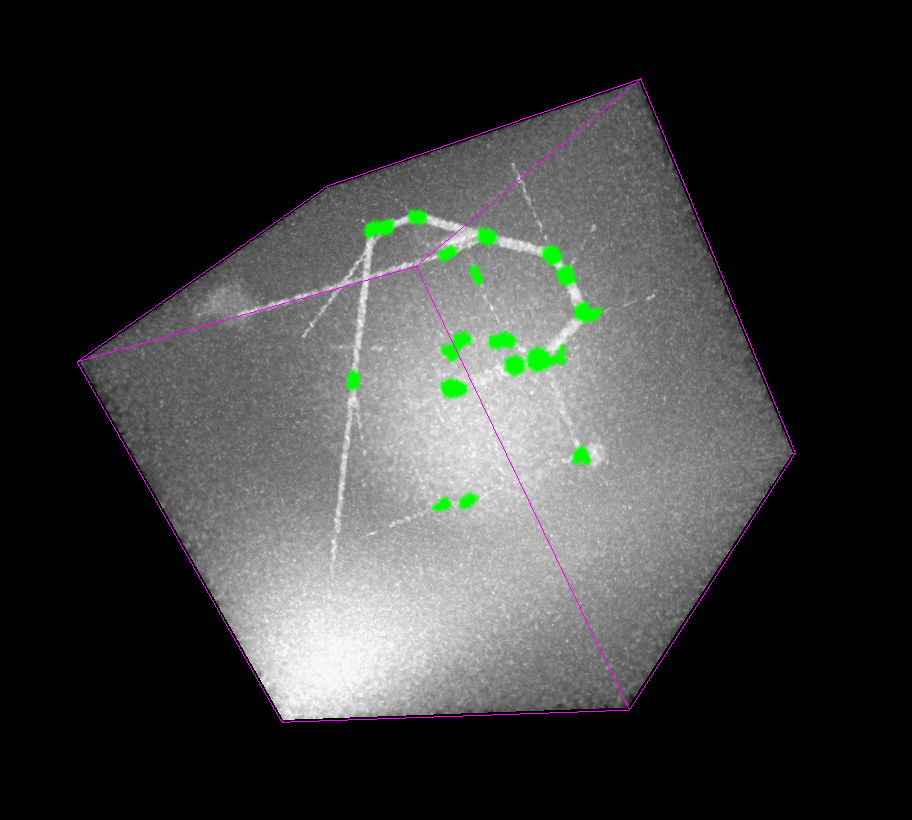
\includegraphics[height=4cm]{Images/exp_seg_gt.png}
    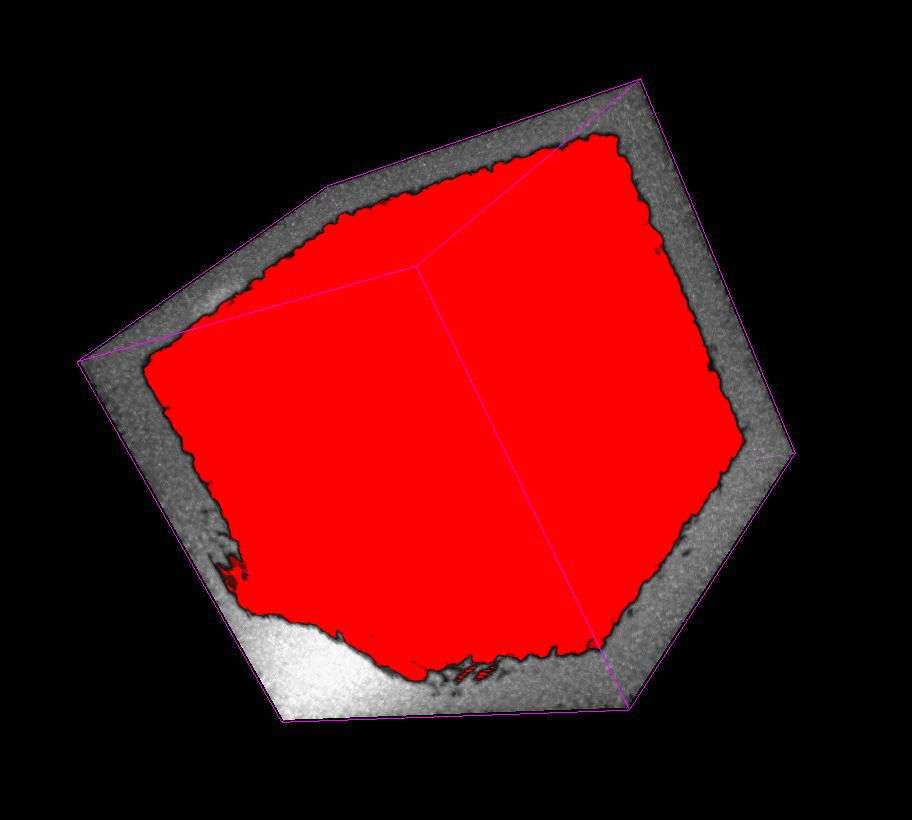
\includegraphics[height=4cm]{Images/exp_seg_40.png}
    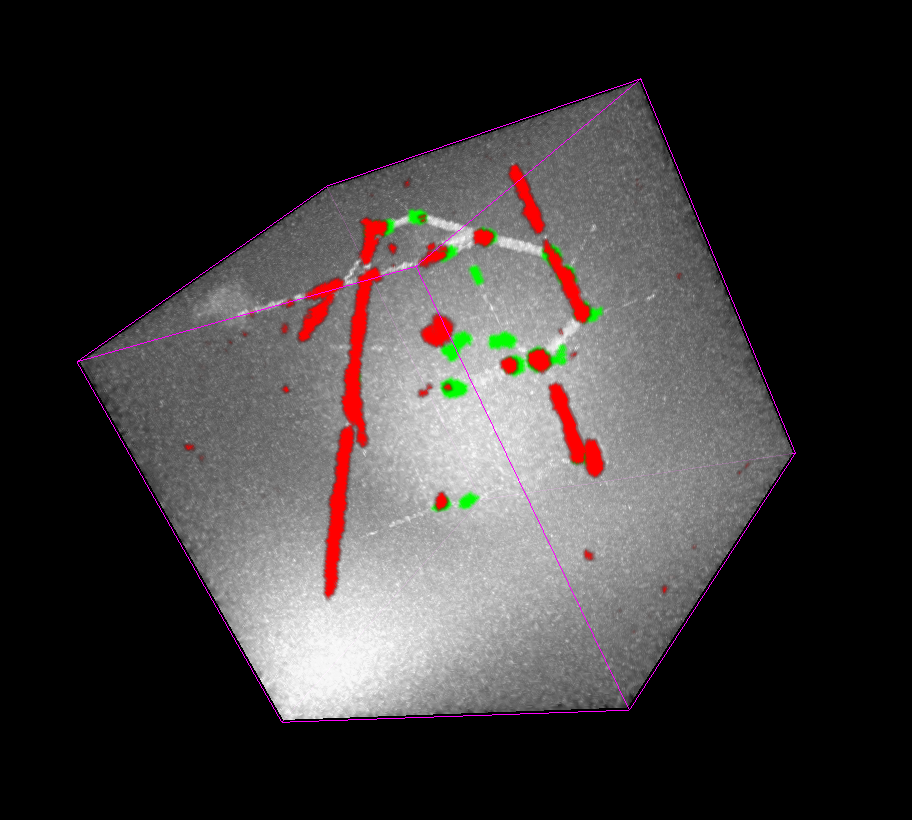
\includegraphics[height=4cm]{Images/exp_seg_100.png}
    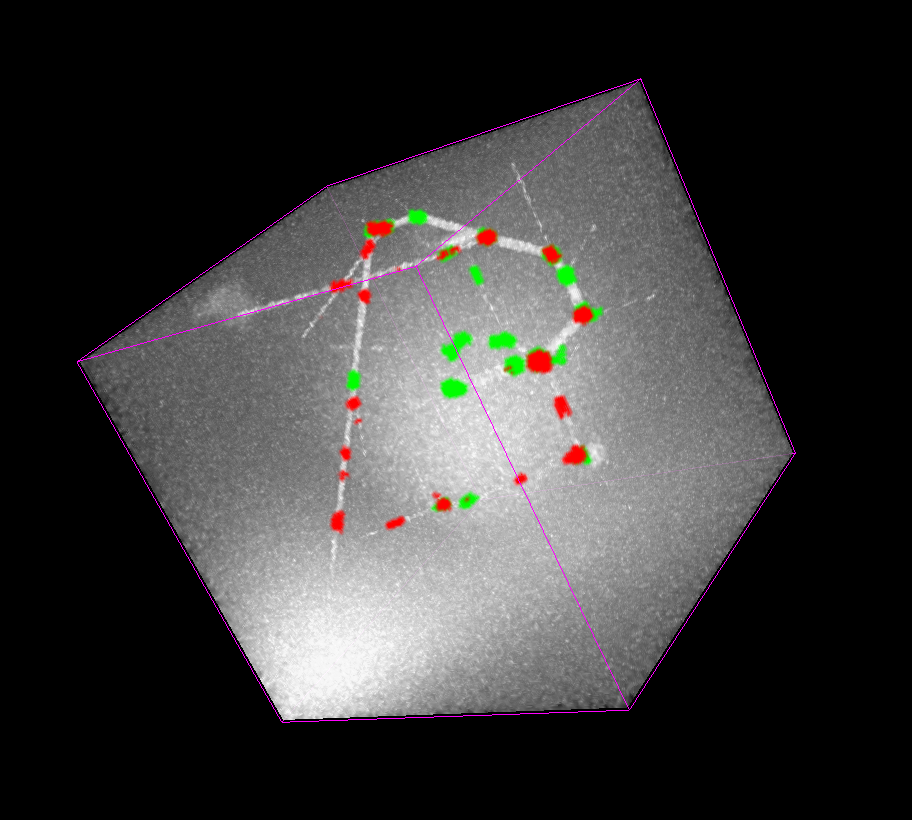
\includegraphics[height=4cm]{Images/exp_seg_200.png}
    \caption{Tentative de segmentation des bifurcations. Inférence à l'itération 40, 100 et 200. Volume en gris, vérités terrain des bifurcations en vert et sortie du réseau en rouge. }
    \label{fig:seg_deep}
\end{figure}

Nous avons ensuite changé d'approche en passant à la classification de patchs contenant une bifurcation ou non. Pour cette classification, nous avons dans un premier temps utilisé des patchs contenant une seule bifurcation dont la position était alignée avec le pixel central des patchs. Nous avons utilisé un réseau de neurones inspiré de l'architecture VGG, c'est-à-dire un réseau avec un encodeur formé de couches convolutionnelles suivi de couches de neurones entièrement connectées. La sortie du réseau est formée d'un seul neurone donnant la probabilité d'appartenance d'un patch à une bifurcation. 

Afin de ne contenir qu'une seule bifurcation par patch, nous avons choisi une taille de $16 \times 16 \times 16$ (Fig. \ref{fig:exp_patchs}). Cette taille impose l'utilisation de réseaux avec peu de couches convolutionnelles car la sortie de ces couches est accompagnée d'une opération de max pooling, qui réduit la taille spatiale du volume d'entrée. 

\begin{figure}[ht]
    \centering
    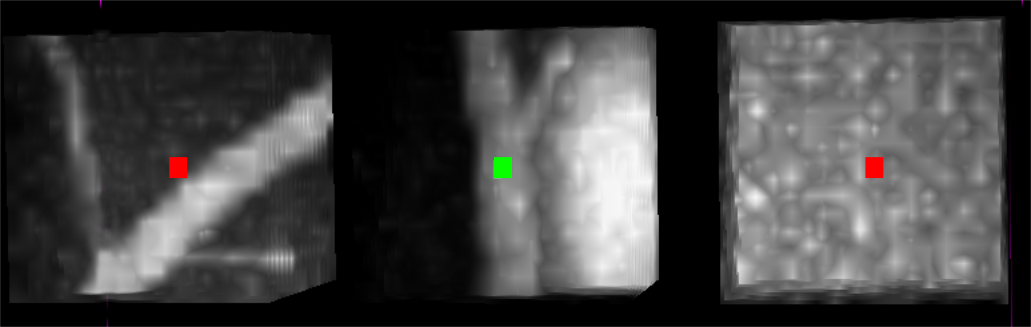
\includegraphics[height=4cm]{Images/exp_patchs_exemple.png}
    \caption{Trois exemples de patchs. Le patch central est un patch positif, les deux autres des patchs négatifs.}
    \label{fig:exp_patchs}
\end{figure}

Les patchs positifs sont tirés aléatoirement dans le volume entier, dans un rayon supérieur à une dizaine de pixels des bifurcations. Nous n'avons pas réussi à faire converger ce premier essai. Nous avons cherché la cause en faisant varier les couches du réseau, ses paramètres (taux d'entrainement, utilisation du pooling ou non) sans succès. Nous avons ensuite augmenté la taille des patchs de $16 \times 16 \times 16$ à $32 \times 32 \times 32$ ce qui a permis au réseau de converger pour la première fois.

Les résultats de classification de patchs étaient relativement corrects, cependant, la classification appliquée à une image complète présentait des résultats très faibles. Nous avons en effet remarqué que le réseau avait tendance à classifier comme bifurcations l'ensemble de l'intérieur des vaisseaux à proximité de la ligne centrale. Une de nos hypothèses a alors été de penser que l'ensemble des bifurcations était un sous ensemble de la ligne centrale. Un réseau apprenant à identifier les lignes centrales aurait une précision très haute de détection des bifurcations, puisque lors de l'entrainement, les patchs négatifs de lignes centrales sont très peu représentés. 

La difficulté a été de construire une méthode pour tirer des patchs proches de la ligne centrale des vaisseaux sans vérité terrain des vaisseaux. En effet, utiliser des informations supplémentaires aurait été à l'encontre des contraintes initiales que nous nous sommes posées. Nous avons donc choisi d'utiliser des filtres de rehaussement pour tirer des patchs dont le pixel central avait une forte probabilité d'appartenir à des vaisseaux. Cette méthode n'a cependant pas réglé le problème des réseaux qui continue à ce jour de classifier l'ensemble de la ligne centrale comme une bifurcation.

\begin{figure}[ht]
    \centering
    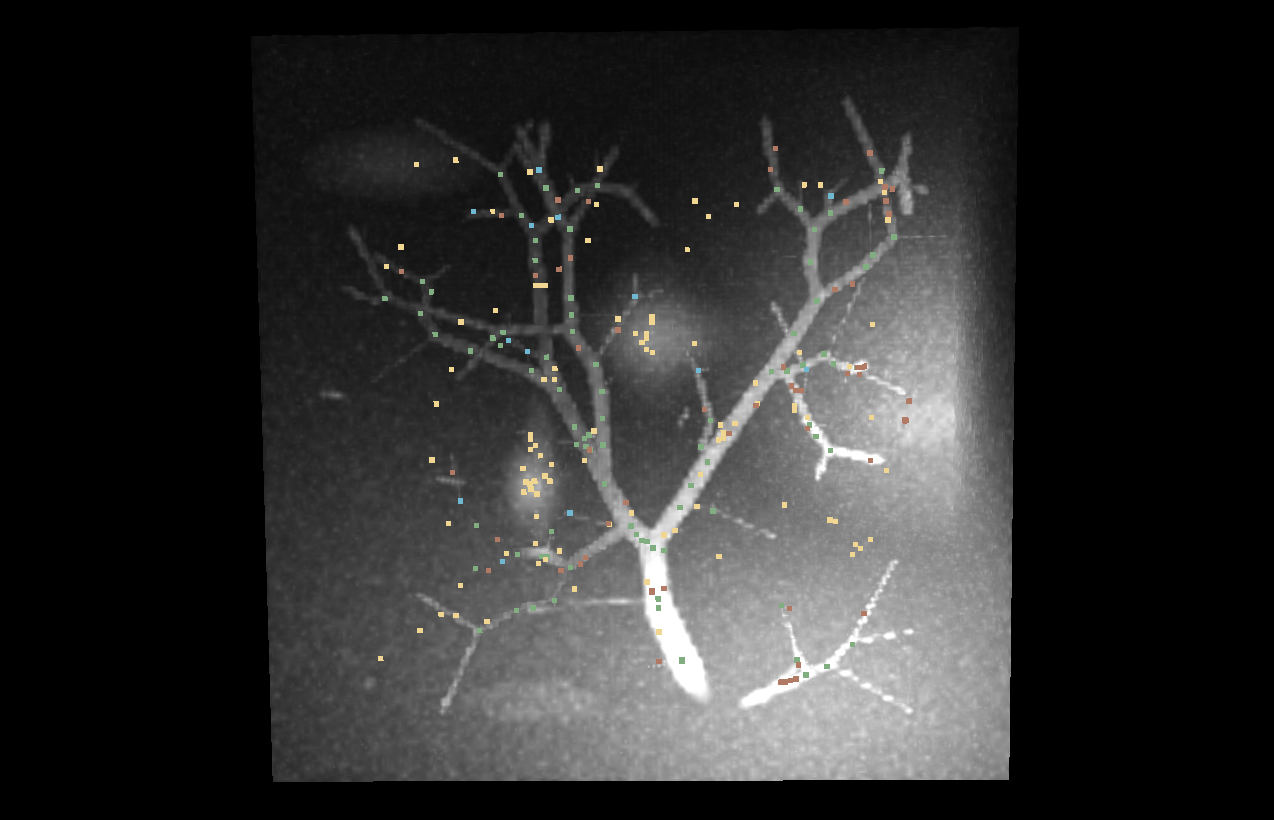
\includegraphics[height=8cm]{Images/exp_bifurcations.png}
    \caption{Exemples de résultats de classifications sur patchs tirés dans un volume. Les points représentent le centre de patchs de taille $32 \times 32 \times 32$ (le volume total fait $128 \times 128 \times 128$ pixels). VN=jaune, VP=vert, FP=bleu, FN=marron.}
    \label{fig:exp_patchs}
\end{figure}

Il est possible que le modèle VGG ne soit pas adapté à la tâche, car le pooling détruit l'information des vaisseaux. Dans un réseau de segmentation de type Unet, les structures fines sont conservées par des skip connections qui ne peuvent pas être mises en place dans ce type dans ce type d'architecture.

\section{ Bilan des travaux}

\todo{Est-ce que la répétition de "nous avons" est dérangeante pour ce résumé de nos contributions ?}

Nous avons articulé l'ensemble de nos travaux de manière à ce qu'ils constituent un socle de connaissances et d'outils pour une personne souhaitant approfondir ses connaissances sur les filtres de rehaussement de vaisseaux. 

Nous avons dans un premier temps établi un état de l'art des filtres de rehaussement recouvrant les vingts dernières années. Nous avons ensuite identifié sept filtres se démarquant de la littérature par la solution proposée pour répondre à des problèmes différents et complémentaires levés par le rehaussement de vaisseaux. Nous avons aussi explicité les différents cadres d'échelles qui permettent au rehaussement d'être efficace sur l'ensemble du réseau vasculaire malgré des variations de taille importantes des vaisseaux.

Nous avons ensuite décidé d'améliorer l'accessibilité des filtres de rehaussement en proposant de rassembler, adapter et réimplémenter les sept filtres dans un cadre commun en C++. Un utilisateur souhaitant utiliser des filtres de rehaussement, peut ainsi éviter de passer par cette étape très chronophage de recherche et d'adaptation de filtres provenant de sources multiples. 

Puis, nous avons proposé un banc de test, permettant de comparer les performances de ces filtres de manière quantitative dans différents contextes. Assez tôt dans sa conception, nous avons fait en sorte que celui-ci soit modulable et extensible par d'autres utilisateurs. Il permet ainsi d'ajouter un nouveau filtre à la base de travail existante qui devient ainsi évolutive, plutôt que de recommencer ex nihilo. Cet outil facilite aussi la démonstration de la pertinence d'une nouvelle contribution.

Les expériences que nous avons menées avec ce banc de test ont mis en valeur les différences significatives entre les filtres de rehaussement. Les filtres hessiens ou de flux proposant des rehaussements lisses, mais parfois surestimés ou rehaussant des bords d'organes. En opposition, RORPO est plus précis dans les structures rehaussées, mais leur aspect est beaucoup plus irrégulier. Les filtres se distinguent aussi par leur résistance au bruit avec des filtres plutôt performants pour de faibles niveaux de bruits, comme Jerman et Sato, mais dont les performances chutent lorsque le bruit augmente. À l'inverse le filtre de Frangi propose un mécanisme intéressant pour le contrôle du bruit.

Nous avons aussi fait en sorte que les implémentations des filtres et du banc de test soient à la fois complémentaires et indépendants. De cette manière, chaque partie peut être réutilisée chacune de son côté. Nous avons d'ailleurs tiré parti de cette propriété en proposant une démonstration en ligne des filtres qui permet de tester, sans installation, les filtres de rehaussement sur des données de l'utilisateur. L'intégration des filtres de rehaussement a aussi été réalisée dans un logiciel de visualisation d'images médicales : 3DSlicer. Les filtres peuvent ainsi être directement utilisés de manière interactive dans celui-ci.

Enfin, pour compenser le manque d'annotations, nous avons participé à l'élaboration d'un pluggin de segmentation, afin que les bases de données hépatiques avec annotations des vaisseaux se démocratisent. Nous avons aussi exploré une méthode de segmentation à partir des seules annotations des bifurcations.

Nous avons finalement élaboré un travail couvrant tous les aspects nécessaires l'étude du rehaussement : le développement des bases de données, la théorie du rehaussement, la mise en pratique des filtres ainsi que leur évaluation.